\subsection{Generate Obfuscation Challenges}
\label{sec:generate}
As shown in Figure~\ref{system}, the first step of \revenge is to generate challenges by first generating random programs and then obfuscating these programs. The generation process can be described as a 5-tuple $\mathit{Gen}$:
\begin{eqnarray}
\label{gentuple}
   \mathit{Gen} & = & 
   (
      \mathit{Script}^1,
      \mathit{Asset},
      \mathit{Seed}^1,
      \mathit{Script}^2,
      \mathit{Seed}^2
   )
\end{eqnarray}
 Together, the elements of this tuple uniquely define the challenges we generate. $\mathit{Gen}$ is kept confidential and it is, essentially, the goal of the reverse engineer to recover the program generated by $\mathit{Gen}$ given only a compiled\footnote{Source code challenges may be provided in the future as well, but compiled binaries tend to better match common real world use cases and thus are more appropriate.} obfuscated binary as input.  

The generation of random programs takes 3 inputs: $\mathit{Asset}$ is the aspect of the program we want to protect (such as a security check or a license check), $\mathit{Script}^1$ sets parameters on the language features to generate (number/size of functions, size of global and local state, kinds of control structures, etc), and $\mathit{Seed}^1$ can be varied to allow us to generate large numbers of unique programs with the same asset, and with the same parameters. In the current version of \revenge, we are asking reverse engineers to {\em de-obfuscate} a challenge, i.e. to transform an obfuscated binary program back into C code. In other words, the asset that they have to recover is the {\em source code} of the program itself. In future work we will extend this to challenges with different types of assets, such as where the goal is to disable a security check or to recover an embedded cryptographic key.

Once programs have been generated, they are obfuscated (point 2 in Figure~\ref{system}). This step takes 3 inputs:  $\mathtt{p}^0.\mathtt{c}$ is the generated plaintext C program, $\mathit{Script}^2$ describes the sequence of obfuscating transformations that should be applied to $\mathtt{p}^0.\mathtt{c}$, and $\mathit{Seed}^2$ can be varied to allow us to generate a diverse set of of uniquely obfuscated programs from the same obfuscation script.

%%%%%%%%%%%%%%%%%%%%%%%%%%%%%%%%%%%%%%%%%%
\subsubsection{Generating Random Programs}
\label{sec:generate:program}
%Generating random programs that are suitable targets for a reverse engineering challenge is a challenging research problem in itself. In order to simulate the most realistic scenario for reverse engineering attacks and isolate the obfuscating effect of the transforms rather than the original program behavior, the program generator should produce programs that exhibit the following traits:
%\begin{enumerate}
%\itemsep-.5em
%\item they should have a simple I/O behavior so that attacks can be easily automated;
%\item they should be complex enough that they cannot be guessed by brute-force examination of their IO behavior;
%\item they should be simple enough that the difficulty of the challenge stems from the complexity of the obfuscation rather than the complexity of the original program;
%\item they should contain unique combinations of control and data structures so that their recovery becomes an interesting challenge;
%\item they should terminate within a reasonable time-bound so that dynamic attacks become feasible;
%\item they should favor automatic or human-assisted automatic attacks over purely manual attacks, as these are the most common in practice;
%\item they should be ``minimal'' (i.e. no smaller program should exhibit the same I/O behavior) to make it obvious when the right de-obfuscated program has been found.
%\end{enumerate}
%Furthermore, the generator must be able to produce an ``infinite'' sequence of different programs.

Generating random programs that are suitable targets for a reverse engineering challenge is a challenging research problem in itself. We extended the \tigress system's program generator to generate simple programs. Each generated function is, essentially, a hash function taking a list of numbers as inputs, and producing a list of numbers as output. A function conceptually consists of three phases: {\em expansion} which seeds a (large) state space from the (small) input, {\em mixing} which introduces control structures (if, while, switch) to update the state space, and {\em contraction} which reduces the state space to the output result. %Figure~\ref{fig:gencode} shows an example. 

To favor automated attacks, in \revenge each challenge consists of multiple unique and obfuscated programs. To be considered successful, a reverse engineer has to solve all of them. In other words, in our current implementation a particular challenge $\mathcal{C}_i$ is generated by 
\begin{align}
\mathcal{C}_i & =  
   \overbrace{
      \{\mathit{Gen}_i, \ldots, \mathit{Gen}_i\}
   }^{n} 
\end{align}   
\begin{align}
   \mathit{Gen}_i & =  
   (
   \mathit{script}_i^\mathrm{gen}, 
   \_, 
   \mathit{rnd}_1, 
   \mathit{script}_i^\mathrm{obf},
   \mathit{rnd}_2
   )
\end{align}
where the $\mathit{rnd}_j$ are pseudo-random numbers and where $n$, the number of obfuscated programs per challenge, is 10.

%\begin{figure}[t]
%\begin{lstlisting}[breaklines=true,basicstyle=\footnotesize,language=C]
%void SECRET(unsigned long input[1] , unsigned long output[1] ) {
%unsigned long state[1] ;
%unsigned long (*output_ref)[1] = output; 
%unsigned int copy15,copy16,copy12 ;
%unsigned short copy17 ; {
% state[0UL] = (input[0UL] << 3UL) | (input[0UL] >> 61UL); // Expansion of the input
% copy12 = *((unsigned int *)(& state[0UL]) + 1);
% *((unsigned int *)(& state[0UL]) + 1) = *((unsigned int *)(& state[0UL]) + 0);
% *((unsigned int *)(& state[0UL]) + 0) = copy12;
% struct timeval __cil_tmp13;
% int __cil_tmp14 = gettimeofday(& __cil_tmp13, 0);// Get the time
% long time = __cil_tmp13.tv_sec;
% if ((state[0UL] >> 4UL) & 1UL) { // Mixing of the state space
%   state[0UL] |= (state[0UL] & 63UL) << 4UL;
%   copy15 = *((unsigned int *)(& state[0UL]) + 0);
%   *((unsigned int *)(& state[0UL]) + 0) = *((unsigned int *)(& state[0UL]) + 1); }
% int failed |= time > 1398629497UL;//This is the time check
% copy17 = *((unsigned short *)(& state[0UL]) + 1); //Contraction to the output
% *((unsigned short *)(& state[0UL]) + 1) = *((unsigned short *)(& state[0UL]) + 2);
% *((unsigned short *)(& state[0UL]) + 2) = copy17
% if (failed) {
%   output_ref = 0UL; // Set pointer to NULL to force crash}
% (*output_ref)[0UL] = state[0UL] >> 1UL; }
%\end{lstlisting}
%\caption{Example of random function generated by \tigress.}
%\label{fig:gencode}
%\end{figure}


%\begin{figure}[t]
%\begin{lstlisting}[breaklines=true,basicstyle=\footnotesize,escapechar=@,language=C]
%@\tigress@ \
%	--Transform=RandomFuns \
%		--RandomFunsName=SECRET \
%		--RandomFunsType=long \
%		--RandomFunsInputSize=1 \
%		--RandomFunsOutputSize=1 \
%		--RandomFunsCodeSize=5 \
%		--RandomFunsLoopSize=2 \
%		--RandomFunsLoopSize=200 \
%\end{lstlisting}
%\caption{Example of challenge generation scripts.}
%\label{fig:scripts1}
%\end{figure}

%\begin{figure}[t]
%\begin{lstlisting}[breaklines=true,basicstyle=\footnotesize,escapechar=@,language=C]
%@\tigress@ \
%	--Transform=Virtualize \
%		--Functions=SECRET_1 \
%		--VirtualizeDispatch=direct \
%		--VirtualizeShortIdents=true \
%		--VirtualizeOperands=stack \
%		--VirtualizeMaxDuplicateOps=1 \
%		--VirtualizeSuperOpsRatio=0.0 \
%		--VirtualizeMaxMergeLength=1 \
%		--VirtualizeNumberOfBogusFuns=0 \
%		--VirtualizeBogusLoopKinds=* \
%		--VirtualizePerformance=IndexedStack \
%		--VirtualizeStackSize=3 \
%\end{lstlisting}
%\caption{Example of challenge obfuscation scripts.}
%\label{fig:scripts2}
%\end{figure}

%%%%%%%%%%%%%%%%%%%%%%%%%%%%%%%%%%%%%%%%%
\subsubsection{Obfuscating Programs}
\revenge uses an obfuscation tool (\tigress) that contains numerous types of obfuscating transformations, with numerous options for each type of transform. %The more powerful transformations are summarized in Table~\ref{tab:tigresstransforms}. 

%\begin{table}[t]
%\centering
%\caption{\tigress Transforms}
%\label{tab:tigresstransforms}
%\begin{tabular}{|p{.3\columnwidth}p{.63\columnwidth}|}
%\toprule
%Transform            & Description                                                                                \\ \midrule
%Virtualize           & Translates a function into virtual machine code that is interpreted at runtime.   \\
%Jit                  & Translates a function into virtual machine code that is compiled to machine code at runtime.         \\
%Dynamic Jit          & Translates a function into binary code which is decoded and re-encoded at runtime (so called {\em dynamic obfuscation}).
%\\
%Flatten              & Removes direct control flow from a function.                                                       \\
%Merge                & Merges two functions into a single function.                                               \\
%Split                & Splits a function into two functions.                                                      \\
%AddOpaque               & Adds bogus control flow to a function.                                                    \\
%EncodeData               & Encodes variables so that their values are hidden at runtime.    \\
%Anti Branch Analysis & Impedes branch analysis using, for example, {\em branch functions}~\cite{linn_CCS_2003}.   \\
%Anti Alias Analysis  & Impedes alias analysis by adding indirect references.                \\
%Anti Taint Analysis  & Impedes dynamic taint analysis by copying variables using, for example, implicit flow~\cite{stephens2018probabilistic}.                                \\ \bottomrule
%\end{tabular}
%\end{table}


\begin{figure}[t]
\centering
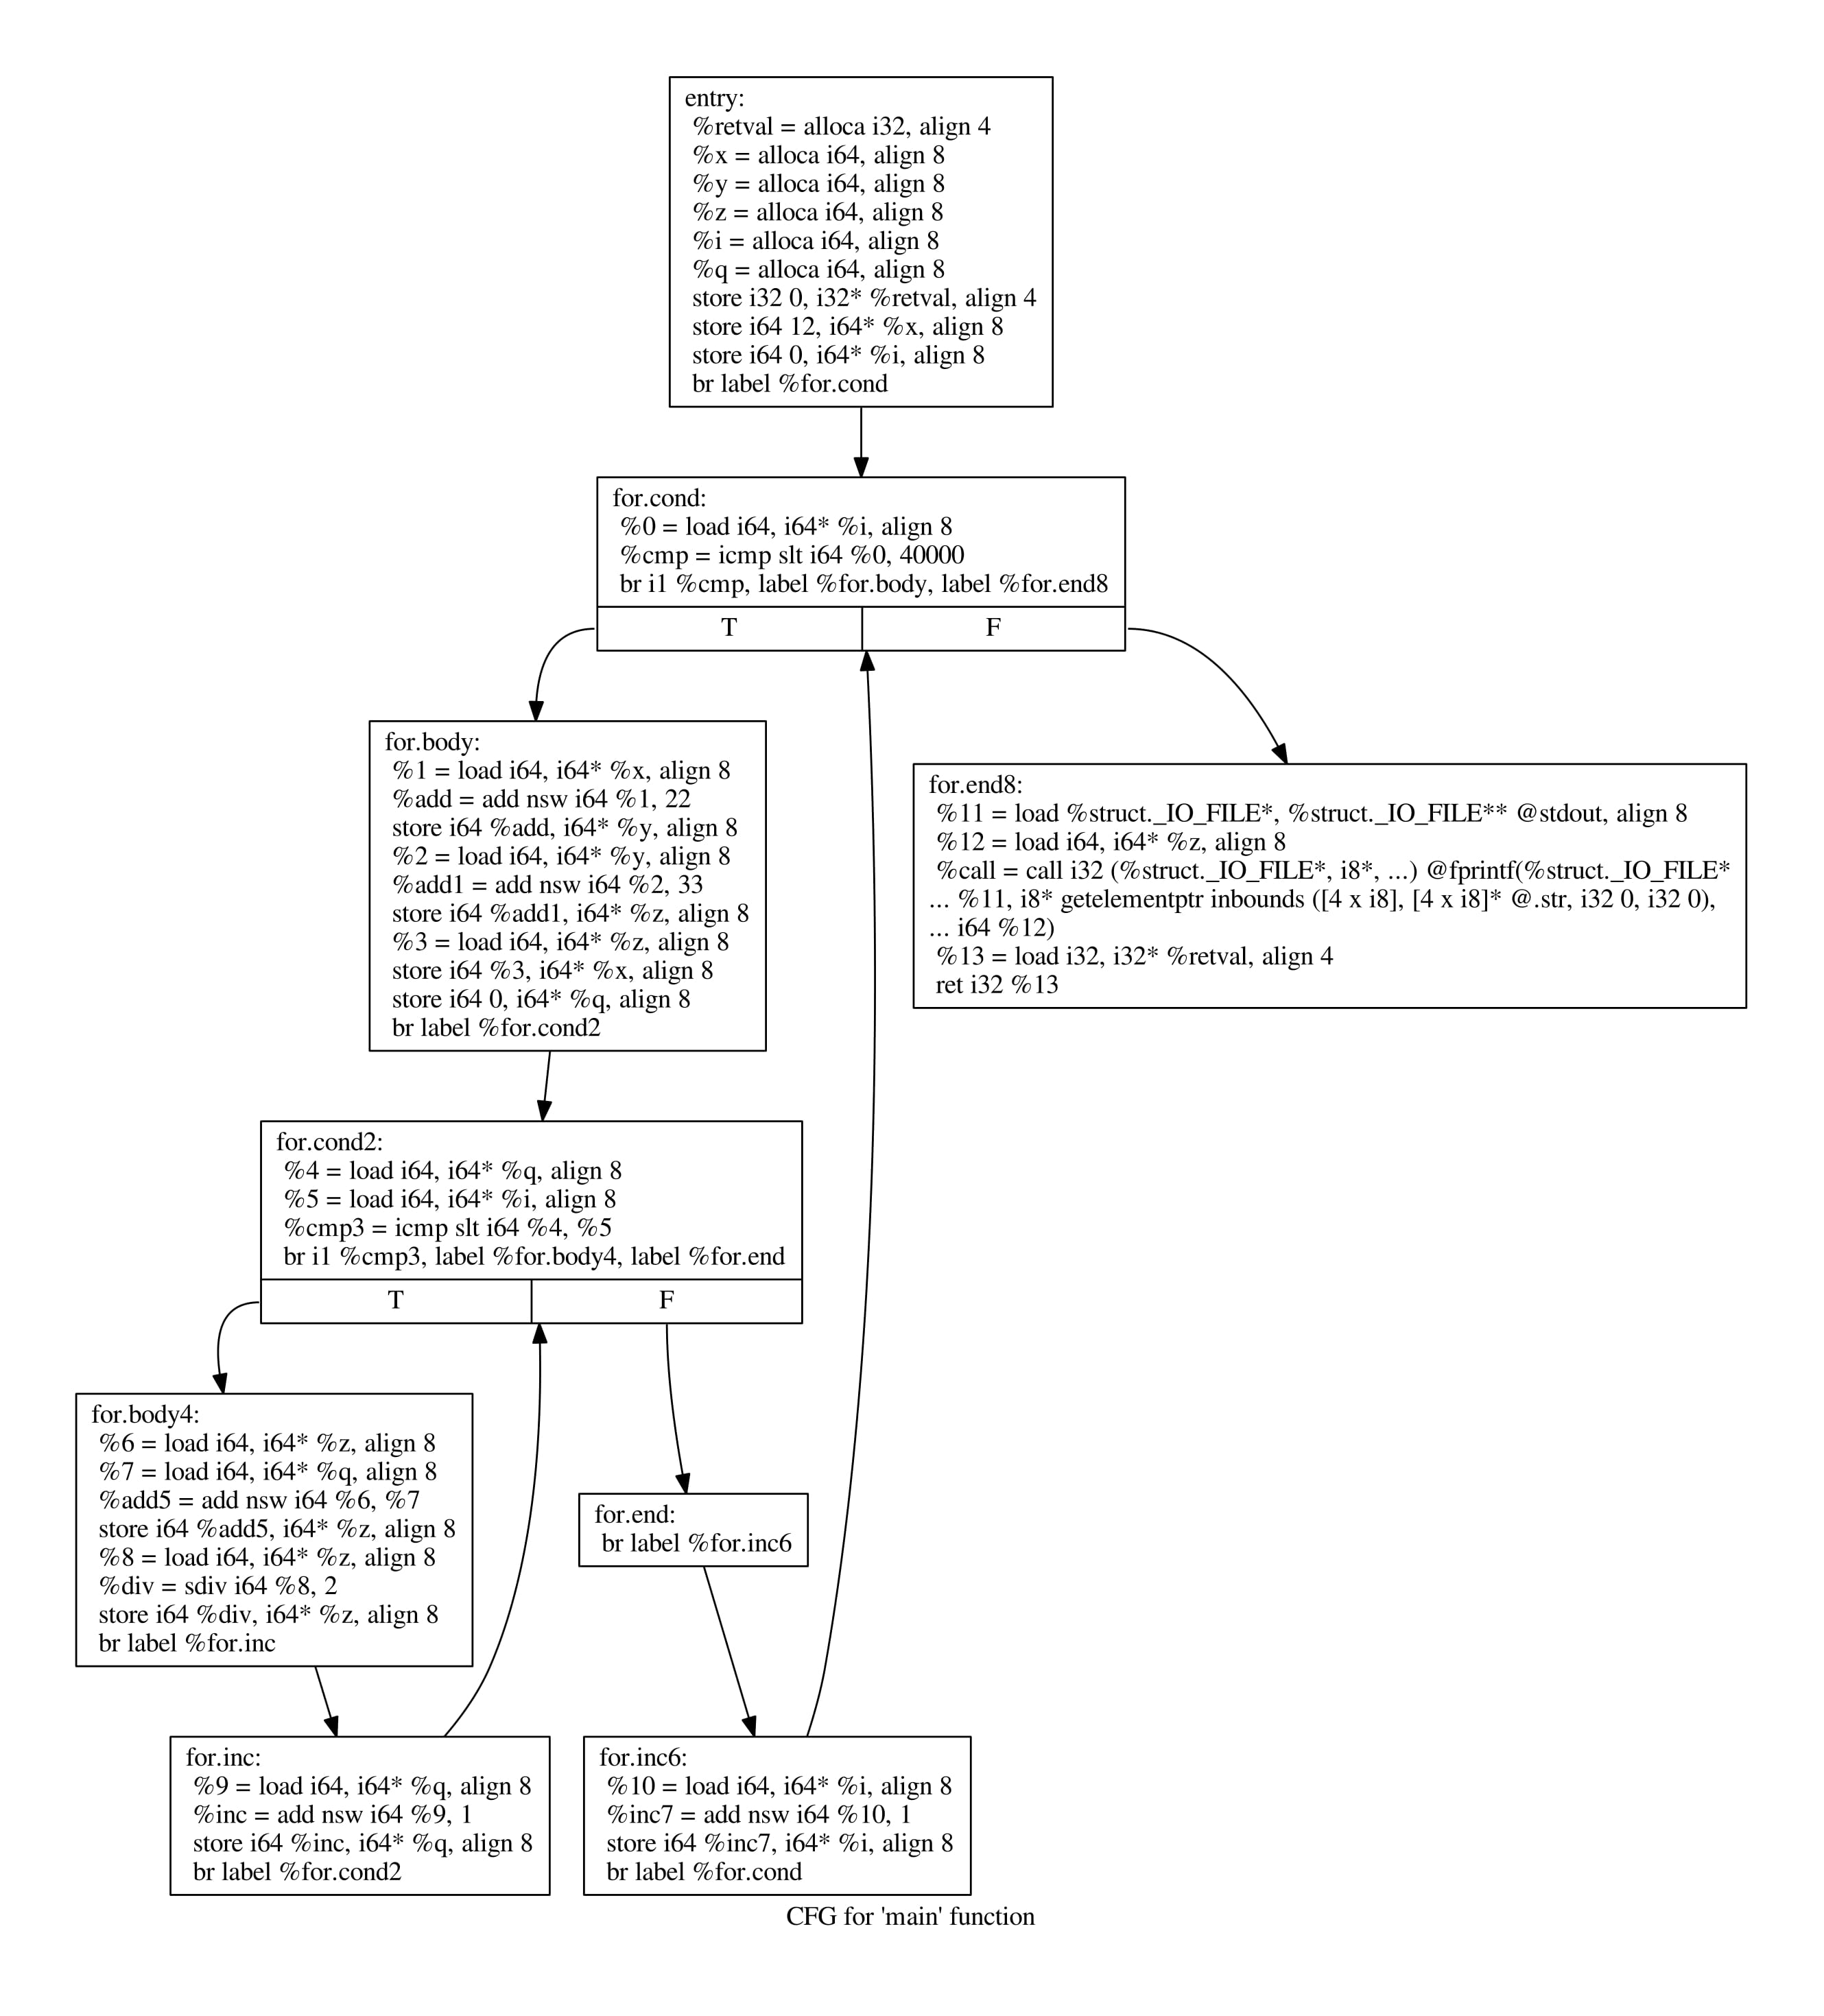
\includegraphics[width=.35\textwidth]{simpleO0_cfg-1.jpg}
\caption{The control flow graph here derives from a simple, sample program with a single loop, a few arithmetic operations, and a print function at the end. LLVM~\cite{lattner2004llvm} compiled this program and generated the control flow graph.}
\label{fig:nonobfcfg}
\end{figure}

\begin{figure}[t]
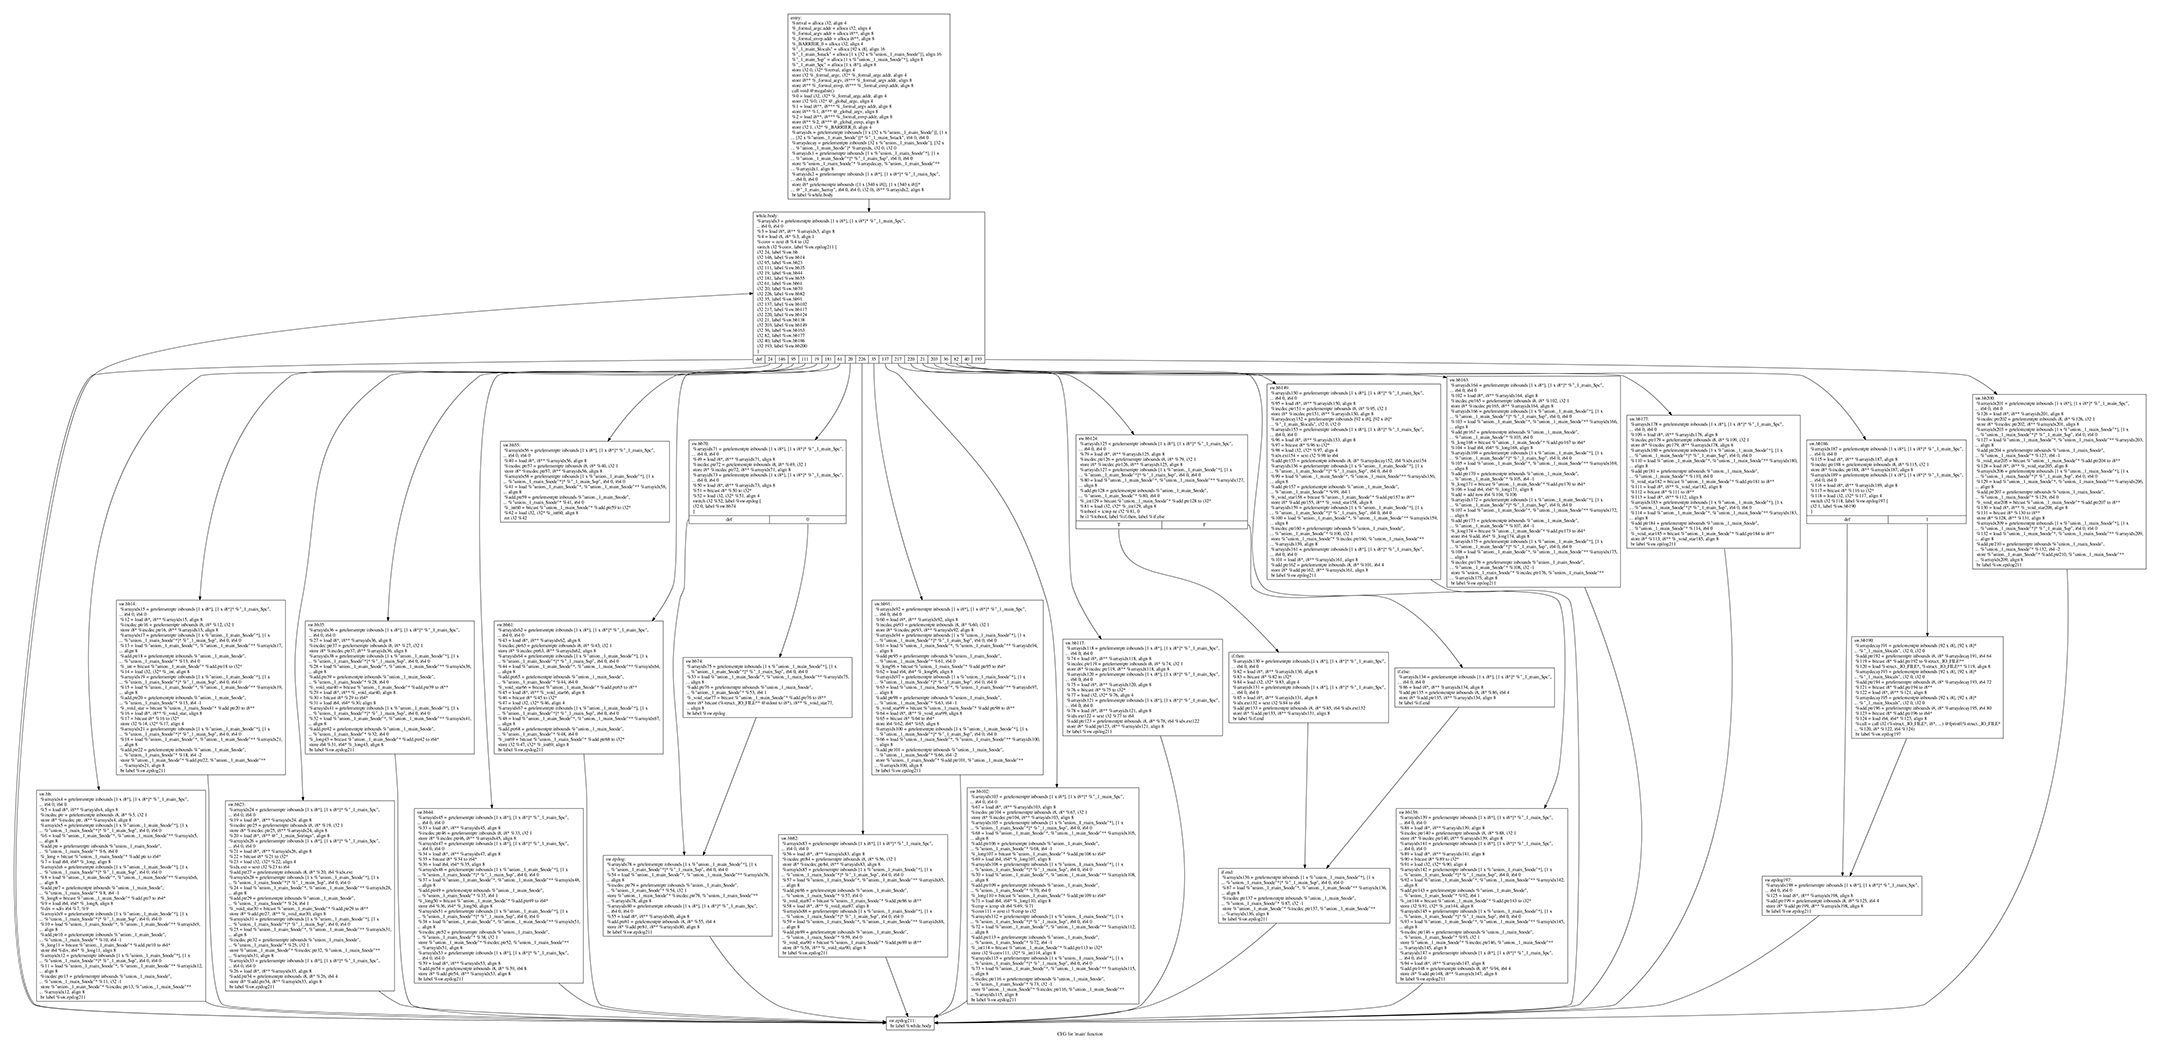
\includegraphics[width=.5\textwidth]{simple_virtualizedO0_cfg-1.jpg}
\caption{This control flow graph resulted from obfuscating the program in Figure~\protect\ref{fig:nonobfcfg} with a virtualization transformation.}
\label{fig:virtcfg}
\end{figure}

As an example of the complexity introduced by obfuscation by virtualization, consider Figure ~\ref{fig:virtcfg} which shows the virtualized version of the program in Figure~\ref{fig:nonobfcfg}.
 
%Virtualization operates by creating a virtual execution unit, paralleling a hardware CPU, in the resulting obfuscated C source.  A given virtualized function consists of a set of virtual instructions.  Control flow is directed through this unit via virtual instructions, which flattens the control flow graph as shown by comparing Figures ~\ref{fig:nonobfcfg} and ~\ref{fig:virtcfg}, which display original and virtualized versions of the same program.  This transform contains many different flags, including a flag which determines how the virtualization handles its dispatch, which determines control flow.  The virtualization transform can further frustrate reverse engineering by being combined with other transforms---opaque predicates masking components such as the virtual program counter expand the potential values, which makes control flow more difficult to predict.  Virtualization makes the operations within a program difficult to follow; each virtual instruction contains some random behavior which can effect various parts of the program in a multitude of ways, such as changing resulting control flow after execution.  Figuring out what part of this execution matters presents a difficult problem; unlike a typical program, the range of possible control flow extends across a much broader range, and many control flow paths may have significant impacts on variables which determine program behavior. 

%The Just-in-Time ("Jit") transform transforms a function into a series of operations which are compiled at runtime.  

%Dynamic Just-in-Time transforms begin with the JIT transform, and constantly modify the resulting instructions at runtime.  
